\begin{frame}{Motivation}
\begin{itemize}
    \item Everyone can probably agree: The AI of today is narrow.
    \item Issues: Generalization, trust, 
    
    \item What motivated my work was the identification of three crucial factors for increased AI capability: Compositionality, communicability, and state abstraction.
\end{itemize}
\end{frame}

\note[itemize]{
    \item As the title of my thesis hints, I'm going to talk about some aspects related to intelligent agents. 
    \item Specifically, I'm going to talk about how programs, as in programming languages, might be useful representations for an agents behavior, and about my research on learning programs.
    \item Another thing I'll be talking about is the value of abstractions, more specifically how causality can help with choosing the right abstractions.
    \item So why should we care about these topics?
    
    \item AI needs to be able to deal with situations outside of those with cheap, plentiful data. Generalize to novel situations that are completely unseen.
    \item Can we trust narrow AI? When?
}

\begin{frame}{Perspective: Robot in a kitchen}
    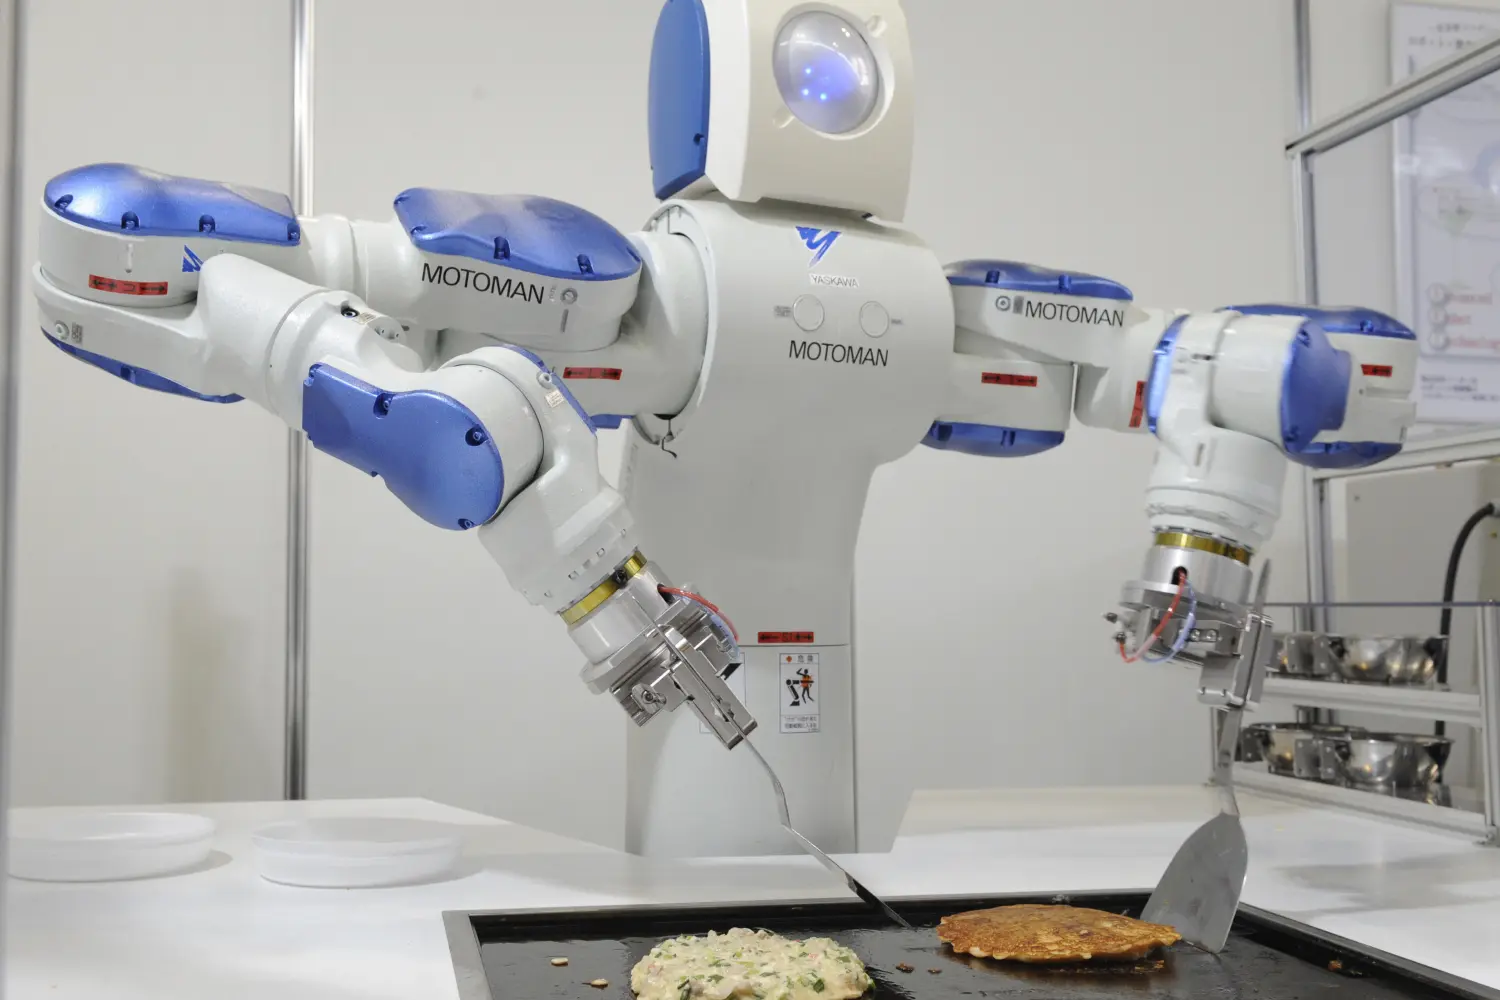
\includegraphics[width=.7\textwidth]{images/robot-cooking.png}
\end{frame}

\note[itemize]{
    \item I'm going to be using references to kitchen scenarios several times
    \item So I wanted to give you an image you could think of whenever I do
    \item These scenarios are relatable yet quite difficult.
    \item Directly motivates the 3 features.
}

\begin{frame}{Composition}
\begin{itemize}
    \item Recipes.
    \item There is never enough data to cover every case in the real world.
    \item 
\end{itemize}
\end{frame}

\note[itemize]{
    \item 
}

\begin{frame}{Communication}
\begin{itemize}
    \item 
    \item 
\end{itemize}
\end{frame}

\begin{frame}{State abstraction}
    \begin{itemize}
        \item 
        \item 
    \end{itemize}
\end{frame}

\begin{frame}{Reinforcement Learning setting}
    \begin{center}
    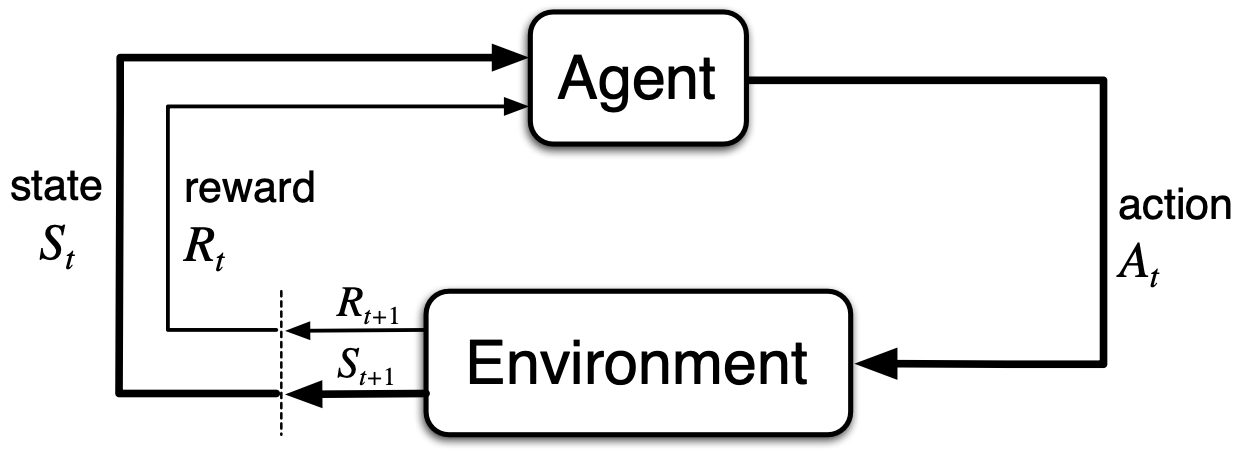
\includegraphics[width=.6\textwidth]{images/rl.png}
    \end{center}
    
    Markov Decision Process $\mathcal{M} = \{\mathcal{S}, \mathcal{A}, P, r, p_0, \gamma\}$, where $\mathcal{S}$ is the state space, $\mathcal{A}$ the action space, $P(s'|s,a)$ is the probabilistic transition function, $r(s,a)$ the reward function, $p_0$ a distribution over initial states, and $\gamma \in (0,1)$ the discount factor.
    
    The goal is to maximize the expected reward, $G_t = \sum_{i=0}^\infty \gamma^i R_{t+i+1}$. 
    
    This is achieved by the policy $\pi(s)$ that optimizes the Bellman equation:
    \begin{equation*}
        v_\pi(s) = \E_\pi\left[R_{t+1} + \gamma G_{t+1} | S_t=s\right].
    \end{equation*}
\end{frame}

\note[itemize]{
    \item 
}

\begin{frame}{Nethack challenge}
    %\centering
    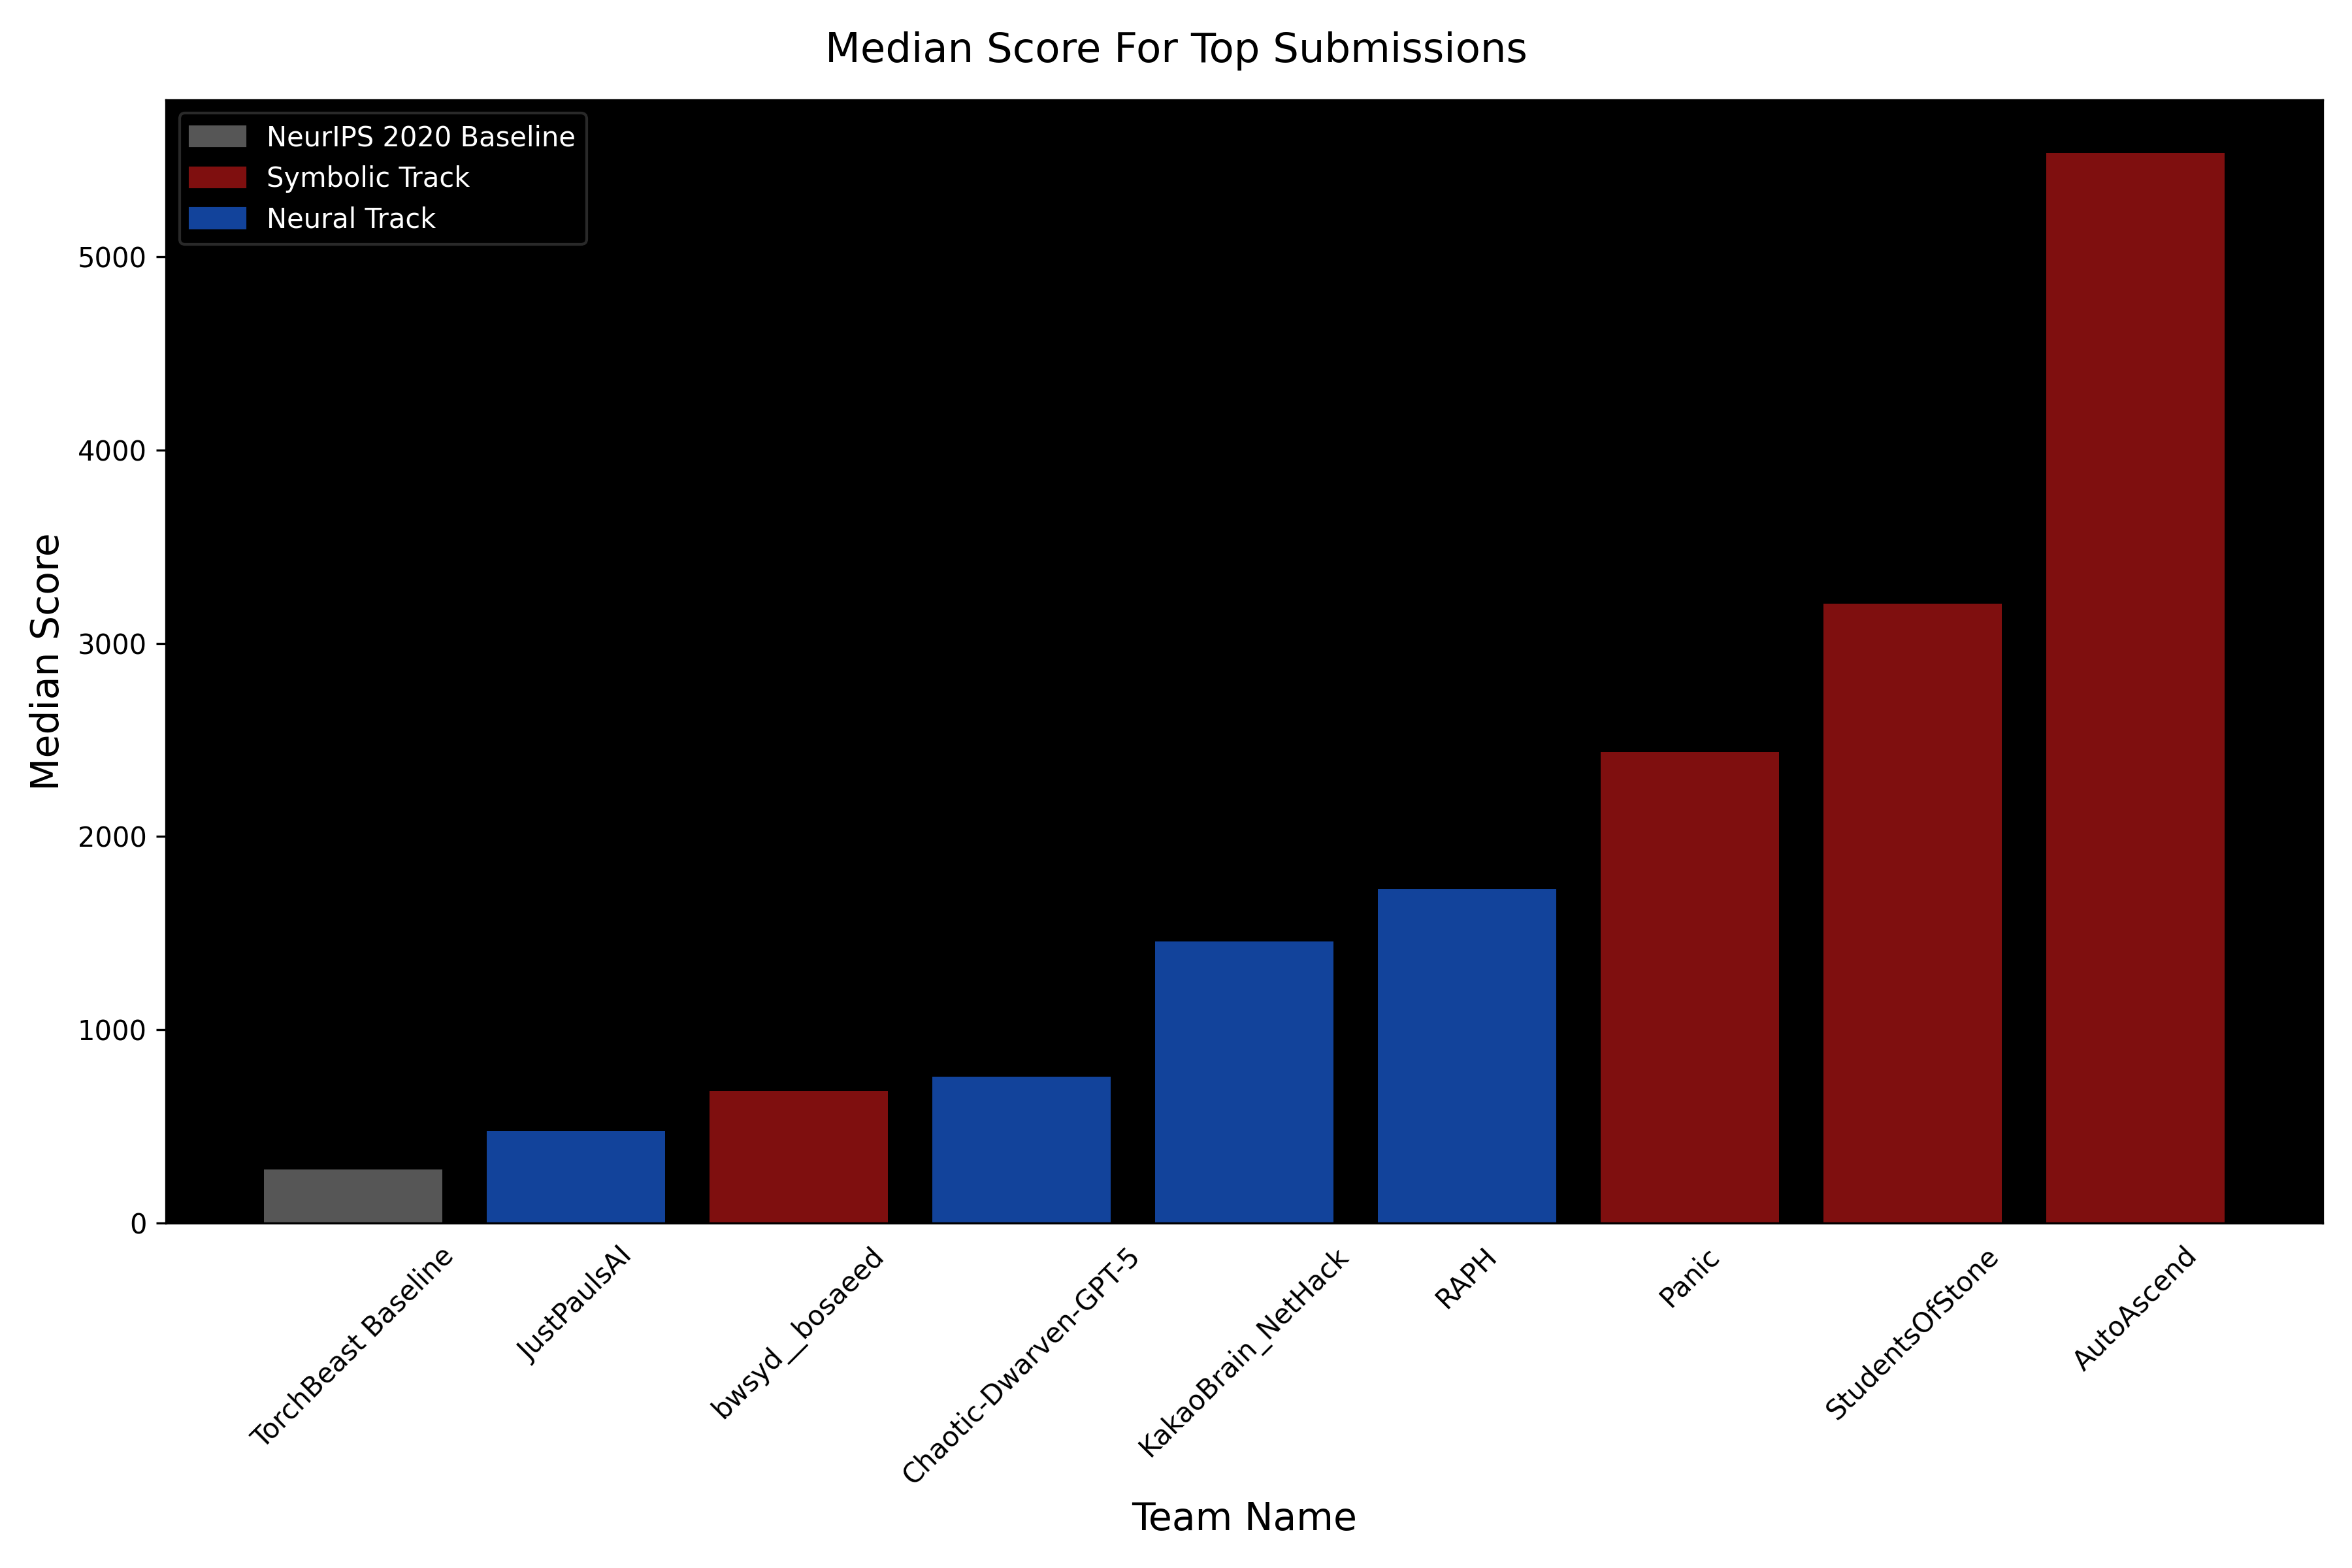
\includegraphics[width=.78\textwidth]{images/FinalScore3.png}
    \mybox{0.7, 0.55}{\fullcite{hambroInsightsNeurIPS20212022}}
\end{frame}

\note[itemize]{
    \item Challenge at NeurIPS 2021, sponsored by Facebook and Deepmind, cash prize.
    \item Roguelike game from 1987, randomly generated levels and widely considered a difficult game even for humans.
    \item Symbolic agents generally beat DL by far - best solution used a hand-coded parser to understand the scene, and hand-coded rule-based hierarchical strategies.
    \item This goes to show that explicitly represented programs are, in some sense, as of 2021 state of the art in representing policies!
    \item It also shows the value of abstraction, since the choice of high-level strategy is based on rules over human-chosen abstracted states.
    \item No agent was remotely close to "winning" the game, though.
}

\begin{frame}{Overview}
    \begin{enumerate}
        \item Programmatic policies, how to represent and learn them.
        \item State abstractions and how to learn them.
    \end{enumerate}
\end{frame}

\note[itemize]{
    \item test1
    \item test2
}